\section{Функции обработчика прерываний от таймера}

Обработчик прерываний таймера запускается в ответ на возникновение аппаратного прерывания таймера, являющегося вторым по приоритету событием в системе (после прерывания по сбою питания). Следовательно, обработчик должен запускаться как можно быстрее, а его время работы желательно сводить к минимуму, чтобы не снижать отзывчивость системы.

\subsection{UNIX}

\subsubsection*{По тику}

\begin{itemize}
	\item инкремент счетчика тиков аппаратного таймера;
	\item обновление таймеров системы (например, переменная lbolt -- хранит количество тиков, отсчитанных с момента загрузки системы);
	\item инкремент счетчика использования процессора текущим процессом (поле p\_cpu структуры proc);
	\item декремент счетчика времени до отправления на выполнение отло­женного вызова (при достижении счетчиком нуля происходит выставление флага для обработчика отложенного вызова);
	\item декремент кванта.
\end{itemize}

\subsubsection*{По главному тику}

\begin{itemize}
	\item регистрация отложенных вызовов функций, от­носящиеся к работе планировщика;
	\item обновление сигналов тревоги и контроль их обработки;
	\item возобновление и управление системными процессами, такими как \textbf{swapper} (производит проверку количества свободной памяти и на основе полученного значения принимает решение о дальнейших действиях) и \textbf{pagedaemon} (выгружает страницы, которые были давно использованы, на диск);

	\item декремент счетчика времени до отправления одного из сигналов:
	
	\begin{itemize}
		\item \textbf{SIGALARM} -- посылается процессу по истечении времени, заданного предварительно функцией alarm();
		\item \textbf{SIGPROF} -- посылается процессу по истечении времени, которое задано в таймере профилирования (общее время выполнения процесса);
		\item \textbf{SIGVTALRM} -- посылается процессу по истечении времени, заданного в <<виртуальном>> таймере (время выполнения процесса в режиме задачи);
	\end{itemize}
	
\end{itemize}

\subsubsection*{По кванту}

\begin{itemize}
	\item 	отправка сигнала \textbf{SIGXCPU} процессу по истечении выделенного ему кванта (при получении данного сигнала процесс прерывает свое выполнение, либо диспетчер выделяет ему еще один квант).
\end{itemize}


\subsection{Windows}

\subsubsection*{По тику}

\begin{itemize}
	\item инкремент счетчика системного времени;
	\item декремент счетчиков отложенных задач;
	\item декремент кванта текущего потока на величину, равную количеству тактов процессора, произошедших за тик (если количество затраченных потоком тактов процессора достигает квантовой цели, запускается обработка истечения кванта);
	\item поставновка объекта в очередь DPC (очередь диспетчера настройки баланса, который активизируется каждую секунду для возможной инициации собы­тий, связанных с планированием и управлением памятью): обработчик ловушки профилирования регистрирует адрес команды, выполнявшейся на момент прерывания.
\end{itemize}

\subsubsection*{По главному тику}

\begin{itemize}
	\item инициализация диспетчера настройки баланса (освобождение объекта <<событие>>, на котором он ожидает).
\end{itemize}

\subsubsection*{По кванту}

\begin{itemize}
	\item инициализация диспетчеризации потоков (постановки соответствующего объекта в очередь DPC).
\end{itemize}

\section{Пересчёт динамических приоритетов}

В операционных системах семейства UNIX и Windows пересчитываться могут только приоритеты \textbf{пользовательских} процессов.

\subsection{UNIX}

Современные ОС семейства UNIX и UNIX-подобные ОС являтся многопоточными. В них единицей диспетчеризачией являются потоки.

В Linux потоки -- "лекговесные процессы". Очередь готовых к выполнению процессов формируется согласно приоритетам процессов и принципу вытесняющего циклического планирования: процессы с одинаковыми приоритетами выполняются в течении кванта времени циклически друг за другом. Если процесс, имеющий более высокий приоритет, поступает в очередь готовых к выполнению, планировщик вытесняет текущий процесс и предоставляет ресурс более приоритетному.

\subsubsection*{Приоритеты процессов}

Приоритет процесса в UNIX задаётся числом в диапазоне от 0 до 127 (чем меньше значение, тем выше приоритет). Приоритеты 0 -- 49 зарезервированы ядром операционной системы, прикладные процессы могут обладать приоритетом в диапазоне от 50 до 127. Приоритеты ядра являются фиксированными величинами.
Приоритеты прикладных задач могут изменяться во времени в зависимости от следующих двух факторов:

\begin{itemize}
	\item фактор любезности процесса -- целое число в диапазоне от 0 до 39 (чем меньше значение фактора любезности, тем выше приоритет процесса; значение 20 по умолчанию); может быть изменён суперпользователем системным вызовом nice;
	
	\item степень загруженности процессора в момент последнего обслуживания процесса.
\end{itemize}

Структура proc содержит следующие поля:

\begin{itemize}
	\item  p\_pri -- текущий приоритет планирования;
	
	\item p\_usrpri -- приоритет режима задачи;
	
	\item p\_cpu -- результат последнего измерения использования процессора;
	
	\item p\_nice -- показатель любезности, устанавливаемый пользователем.
\end{itemize}

Планировщик использует поле p\_pri для принятия решения о том, какой процесс отправить на выполнение. Значения полей p\_pri и p\_usrpri одинаковы, когда процесс находится в режиме задачи. Когда процесс просыпается после блокировки в системном вызове, его приоритет временно повышается. Планировщик использует p\_usrpri для хранения приоритета, который будет назначен процессу при переходе из режима ядра в режим задачи, а p\_pri – для хранения временного приоритета для выполнения в режиме ядра.

Ядро связывает приоритет сна (0 -- 49) с событием или ожидаемым ресурсом, из-за которого процесс может быть заблокирован. Когда блокированный процесс просыпается, ядро устанавливает p\_pri, равное приоритету сна события или ресурса, на котором он был заблокирован, следовательно, такой процесс будет назначен на выполнение раньше, чем другие процессы в режиме задачи.

В таблице 2.1 приведены значения приоритетов сна для систем 4.3BSD UNIX и SCO UNIX. 

\begin{figure}[h!]
	\centering
	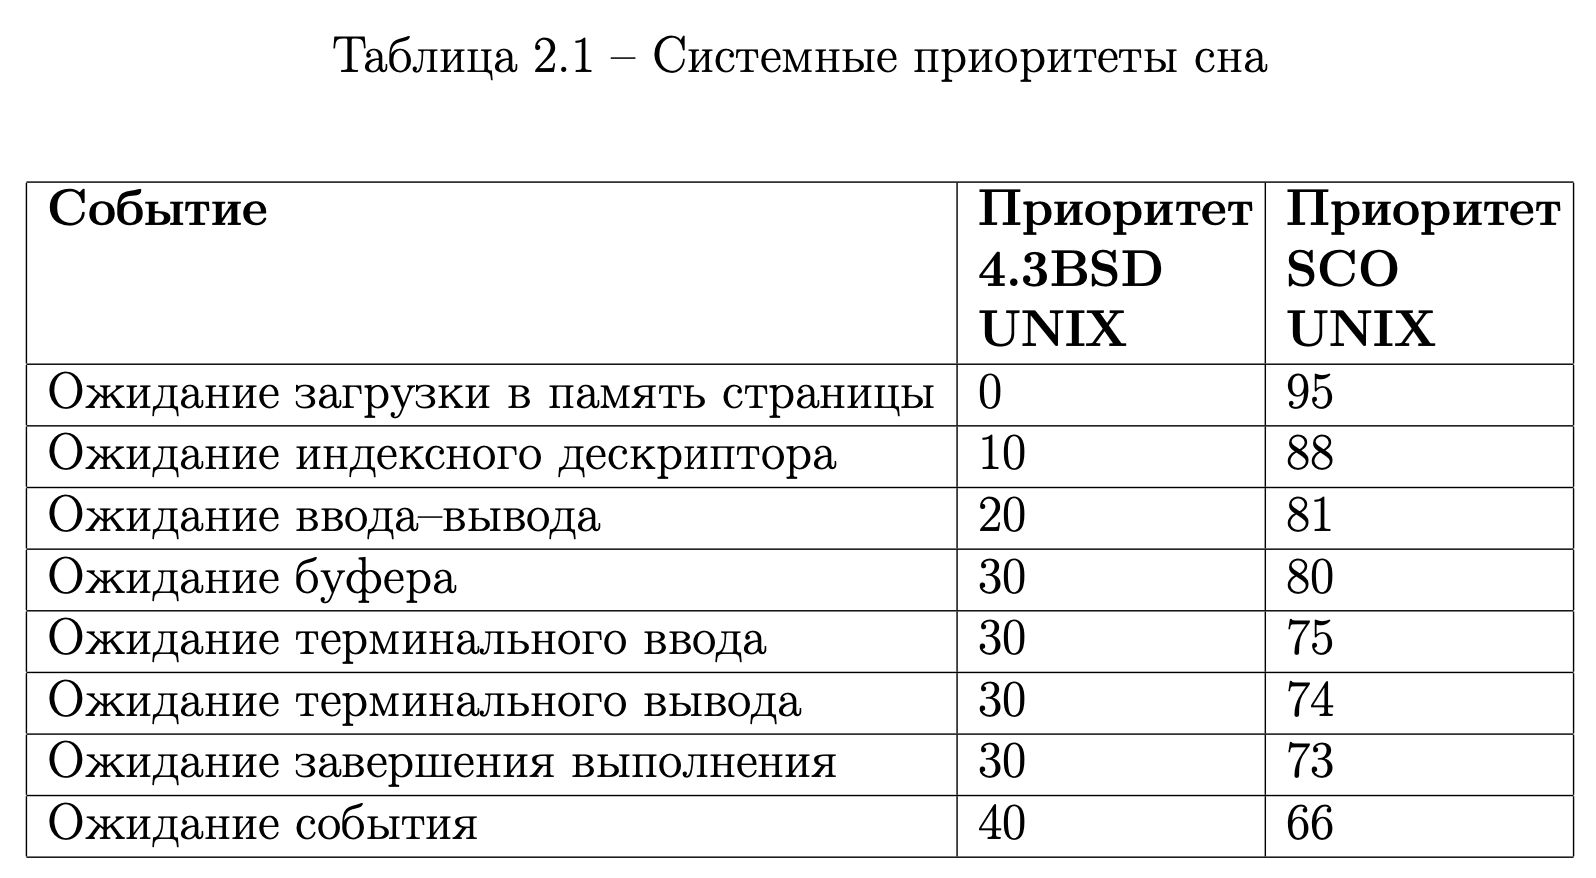
\includegraphics[scale=1.0, width=0.85\textwidth]{assets/table}
\end{figure}

Такой подход позволяет системным вызовам быстрее завершать свою работу. По завершении процессом системного вызова его приоритет сбрасывается в значение текущего приоритета в режиме задачи. Если при этом приоритет окажется ниже, чем приоритет другого запущенного процесса, ядро произведет переключение контекста.

Приоритет в режиме задачи зависит от фактора любезности и последней измеренной величины использования процессора. 
Системы разделения времени стараются выделить процессорное время таким образом, чтобы все процессы системы получили его в равных количествах, что требует слежения за использованием процессора.

Поле p\_cpu содержит величину последнего измерения использования процессора процессом. При создании процесса это поле инициализируется нулем. На каждом тике обработчик таймера увеличивает p\_cpu на единицу для текущего процесса, вплоть до максимального значения -- 127. Каждую секунду ядро вызывает процедуру schedcpu, которая уменьшает значение p\_cpu каждого процесса исходя из фактора <<полураспада>>.

В 4.3BSD для расчета применяется формула:

\begin{center}
	\( d = \frac{2 \cdot la}{2 \cdot la + 1} \),
\end{center}
где la -- load\_average -- это среднее количество процессов в состоянии готовности за последнюю секунду.

Кроме того, процедура schedcpu также пересчитывает приоритеты режима задачи всех процессов по формуле

\begin{center}
	\( p_{\text{usrpri}} = PUSER + \frac{p{\text{\_cpu}}}{4} + 2 \cdot p{\text{\_nice}} \),
\end{center}
где PUSER -- базовый приоритет в режиме задачи, равный 50.

Если процесс до вытеснения другим процессом использовал большое количество процессорного времени, его p\_cpu будет увеличен, что приведет к увеличению значения p\_usrpri и к понижению приоритета.

Чем дольше процесс простаивает в очереди на выполнение, тем меньше его p\_cpu. Это позволяет предотвратить зависания низкоприоритетных процессов. 
Если процесс большую часть времени выполнения тратит на ожидание ввода--вывода, то он остается с высоким приоритетом.

Системы разделения времени пытаются выделить процессорное время таким образом, чтобы конкурирующие процессы получили его примерно в равных количествах. Фактор <<полураспада>> обеспечивает экспоненциально взвешанное среднее значение использования процессора в течение функционирования процесса. Формула, применяемая в SVR3 имеет недостаток: вычисляя простое экспоненциальное среднее, она способствует росту приоритетов при увеличении загрузки системы.

\subsection{Windows}

В системе Windows при создании процесса ему назначается приоритет, который является базовым для потоков процесса и его потомков.  

В Windows реализовано вытесняющее планирование на основе уровней приоритета, при которой выполняется готовый поток с наивысшим приоритетом.

Если поток с более высоким приоритетом готов к выполнению, текущий поток вытесняется планировщиком, даже если квант текущего потока не истёк.

В Windows за планирование отвечает совокупность процедур ядра, называемая диспетчером ядра. Диспетчеризация может быть вызвана, если:

\begin{itemize}
\item поток готов к выполнению;
\item истёк квант текущего потока;
\item поток завершается или переходит в состояние ожидания;
\item изменился приоритет потока;
\item изменилась привязка потока к процессору.
\end{itemize}

\subsubsection*{Приоритеты процессов}

В системе предусмотрено 32 уровня приоритетов: уровни реального времени (16–31), динамические уровни (1–15) и системный уровень (0).

Процесс по умолчанию наследует свой базовый приоритет у того процесса, который его создал. Затем назначается относительный приоритет потоков в рамках процессов. Уровни приоритета потоков назначаются Windows API и ядром операционной системы.

Windows API сортирует процессы по классам приоритета, которые были назначены при их создании:

\begin{itemize}
	\item реального времени (real-time (4));
 	\item высокий (high (3));
	\item выше обычного (above normal (6));
	\item обычный (normal (2));
	\item ниже обычного (below normal (5));
	\item простой (idle (1)).
\end{itemize}

\subsubsection*{Приоритеты потоков}

Затем назначается относительный приоритет потоков в рамках процессов:

\begin{itemize}
	\item критичный по времени (time critical (15));
	\item наивысший (highest (2));
	\item выше обычного (above normal (1));
	\item  обычный (normal (0));
	\item ниже обычного (below normal (-1));
	\item низший (lowest (-2));
	\item простой (idle (-15))
\end{itemize}

Относительный приоритет -- это приращение к базовому приоритету процесса.

C точки зрения планировщика Windows важно только значение приоритета. Процесс обладает только базовым приоритетом, тогда как поток имеет базовый, который наследуется от приоритета процесса, и текущий приоритет. Процесс по умолчанию наследует свой базовый приоритет у того процесса, который его создал.

Операционная система может на короткие интервалы времени повышать приоритеты потоков из динамического диапазона, но никогда не регулирует приоритеты потоков в диапазоне реального времени. Приложения пользователя обычно запускаются с базовым приоритетом normal. Некоторые системные процессы имеют приоритет выше 8, что гарантирует, что потоки в этих процессах будут запускаться с более высоким приоритетом.

Соответствие между приоритетами Windows API и ядра системы приведено в таблице 2.2.

\begin{figure}[h!]
	\centering
	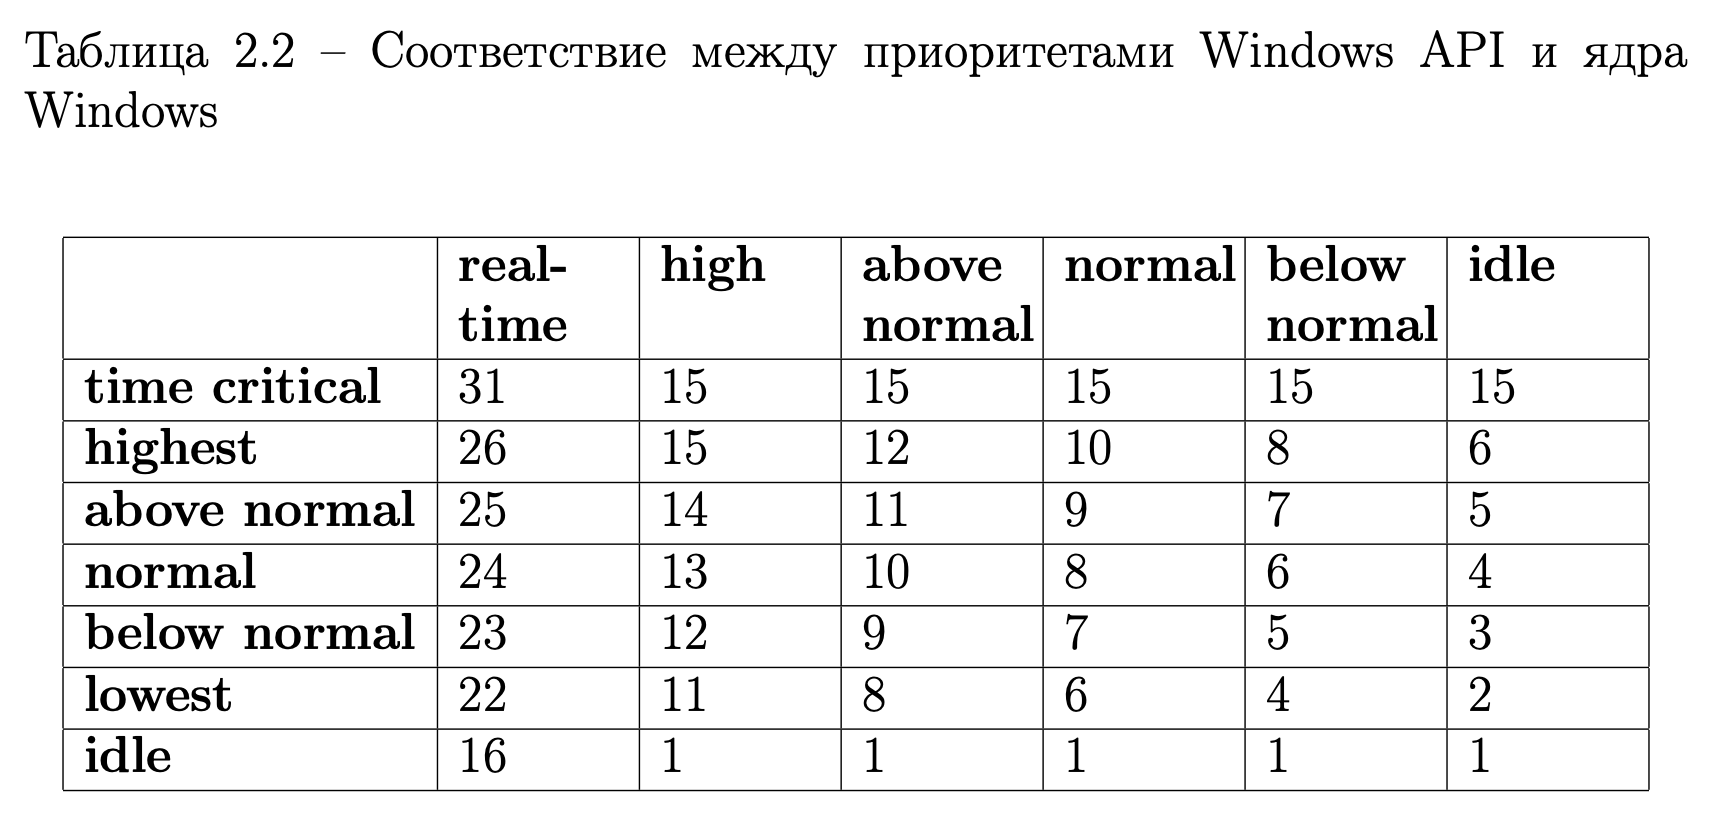
\includegraphics[scale=1.0, width=1.0\textwidth]{assets/table-2}
\end{figure}

Система динамически повышает приоритет текущего потока в следующих случаях:

\begin{itemize}
	\item по завершении операции ввода-вывода;
	\item  по окончании ожидания на событии или семафоре исполнительной системы;
	\item по окончании ожидания потоками активного процесса;
	\item при пробуждении GUI-потоков из-за операции с окнами;
	\item если поток, готовый к выполнению, задерживается из-за нехватки процессорного времени.
\end{itemize}

Динамическое повышение приоритета применяется только к потокам из динамического диапазона (1--15). Приоритет потока не может оказаться выше 15. 

\subsubsection*{Повышение приоритета по завершении операции ввода-вывода}

По окончании определенных операций ввода-вывода Windows временно повышает приоритет потоков и потоки, ожидающие завершения этих операций, имеют больше шансов возобновить выполнение и обработать полученные от устройств ввода-вывода данные.

Драйвер устройства ввода-вывода через функцию IoCompleteRequest указывает на необходимость динамического повышения приоритета после выполнения соответствующего запроса.

В таблице 2.3 приведены приращения приоритетов.

\begin{figure}[h!]
	\centering
	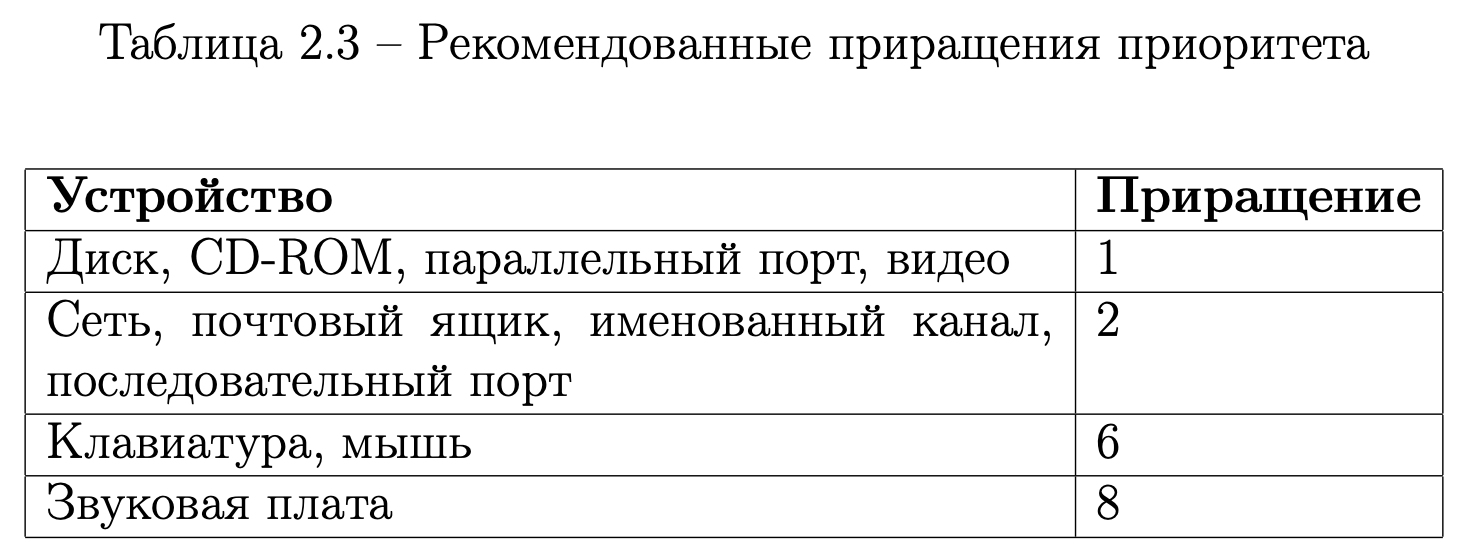
\includegraphics[scale=1.0, width=0.85\textwidth]{assets/table-3}
\end{figure}


Приоритет потока повышается относительно базового приоритета. На рисунке 2.1 показано, что после повышения приоритета поток в течение одного кванта выполняется с повышенным приоритетом, а затем приоритет снижается на один уровень с каждым последующим квантом. Цикл продолжается до тех пор, пока приоритет не снизится до базового.

\begin{figure}[h!]
	\centering
	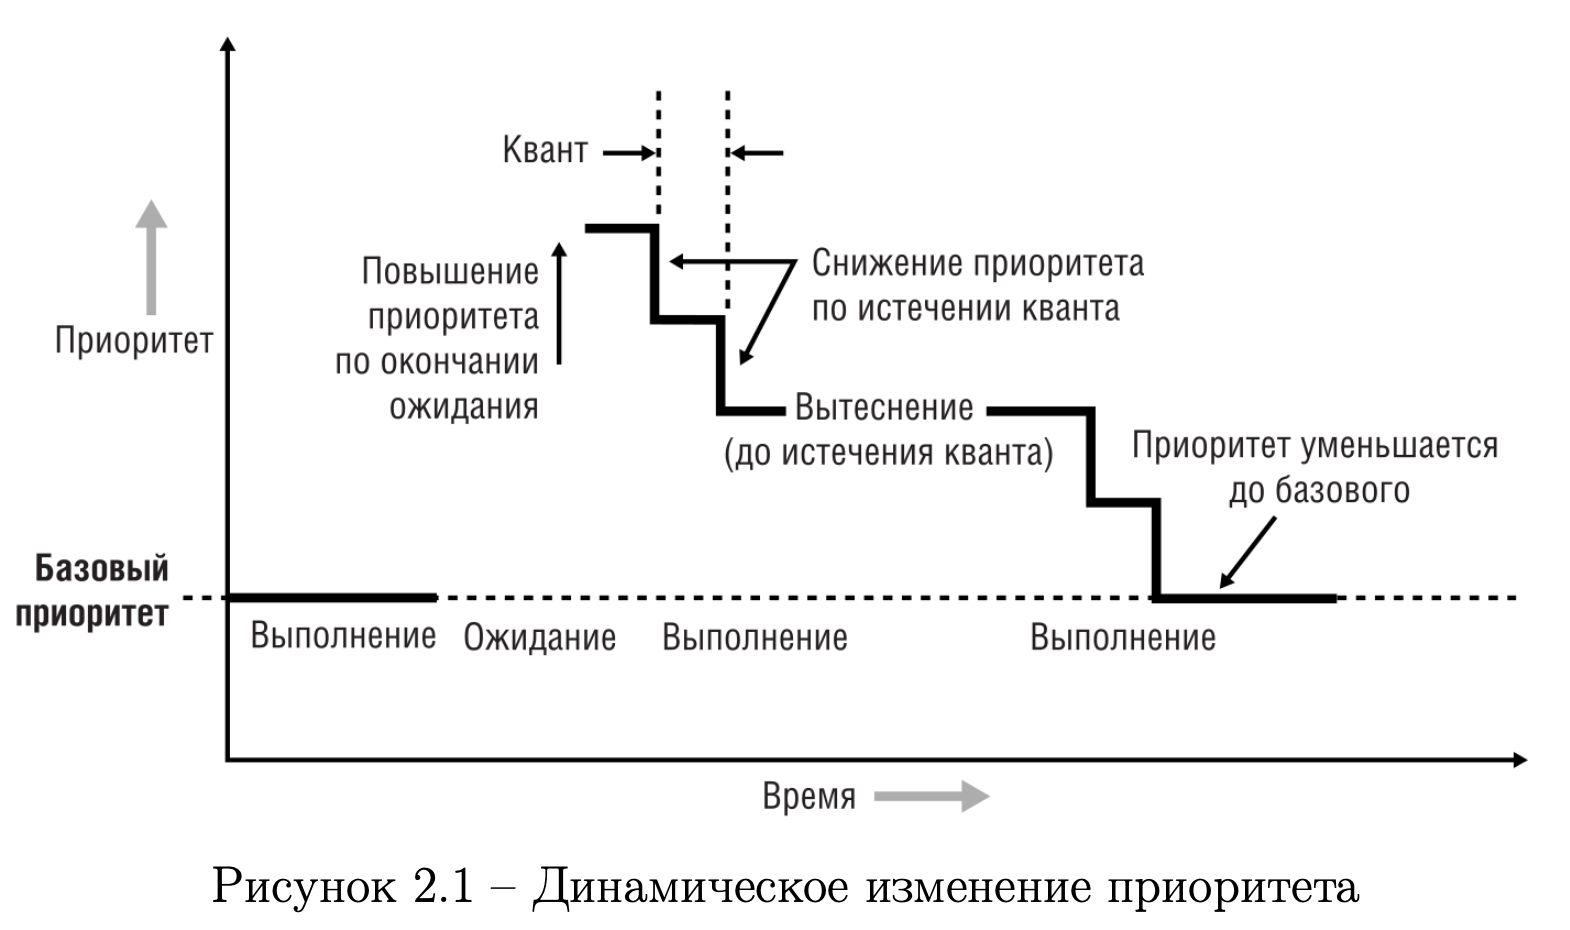
\includegraphics[scale=1.0, width=0.75\textwidth]{assets/img-4}
\end{figure}

\subsubsection*{Повышение приоритета по окончании ожидания на событии или семафоре}

Если ожидание потока на событии системы или семафоре успешно завершается из-за вы SetEvent, PulseEvent или ReleaseSemaphore, его приоритет повышается на 1. Такая регулировка позволяет равномернее распределить процессорное время -- потокам, блокируемым на событиях, процессорное время требуется реже, чем остальным. В данном случае действуют те же правила динамического повышения приоритета. 

К потокам, пробуждающимся в результате установки события вызовом функций NtSetEventBoostPriority и KeSetEventBoostPriority, повышение приоритета применяется особым образом.

\subsubsection*{Повышение приоритета по окончании ожидания потоками активного процесса}

Если поток в активном процессе завершает ожидание на объекте ядра, функция ядра KiUnwaitThread повышает его текущий приоритет на величину значения PsPrioritySeparation -- это индекс в таблице квантов, с помощью которой выбираются величины квантов для потоков активных процессов. Какой процесс является в данный момент активным, определяет подсистема управления окнами.

Приоритет повышается для создания преимуществ интерактивным приложениям по окончании ожидания, в результате чего повышаются шансы на возобновление потока приложения. Важной особенностью данного вида динамического повышения приоритета является то, что он поддерживается всеми системами Windows и не может быть отключен даже функцией SetThreadPriorityBoost.

\subsubsection*{Повышение приоритета при пробуждении GUI- потоков}

Приоритет потоков окон пользовательского интерфейса повышается на 2 после их пробуждения из-за активности подсистемы управления окнами. Приоритет повышается по той же причине, что и в предыдущем случае, -- для увеличения отзывчивости интерактивных приложений.

\subsubsection*{Повышение приоритета при нехватке процессорного времени}


Раз в секунду диспетчер настройки баланса -- системный поток, предназначенный для выполнения функций управления памятью – сканирует очереди готовых потоков и ищет потоки, которые находятся в состоянии готовности в течение примерно 4 секунд. Диспетчер настройки баланса повышает приоритет таких потоков до 15. Причем в Windows 2000 и Windows XP квант потока удваивается относительно кванта процесса, а в Windows Server 2003 квант устанавливается равным 4 единицам. По истечении кванта приоритет потока снижается до исходного уровня. Если потоку все еще не хватило процессорного времени, то после снижения приоритета он возвращается в очередь готовых процессов. Через 4 секунды он может снова получить повышение приоритета.

Чтобы свести к минимуму расход процессорного времени, диспетчер настройки баланса сканирует только 16 готовых потоков за раз, а повышает приоритет не более чем у 10 потоков за раз. Диспетчер настройки баланса не решает всех проблем с приоритетами потоков, однако позволяет потокам, которым не хватает процессорного времени, получить его.

